% UG project example file, February 2022
%  A minior change in citation, September 2023 [HS]
% Do not change the first two lines of code, except you may delete "logo," if causing problems.
% Understand any problems and seek approval before assuming it's ok to remove ugcheck.
\documentclass[logo,bsc,singlespacing,parskip]{infthesis}
\usepackage{ugcheck}

% Include any packages you need below, but don't include any that change the page
% layout or style of the dissertation. By including the ugcheck package above,
% you should catch most accidental changes of page layout though.

\usepackage{microtype} % recommended, but you can remove if it causes problems
\usepackage{natbib} % recommended for citations

\usepackage{enumitem}
\usepackage{tikz}
\usepackage{graphicx}\usetikzlibrary{shapes.geometric, arrows}

\begin{document}
\begin{preliminary}

\title{Out-of-core Multi-resolution Gaussian Splatting Optimization Pipeline for Large Scale Scene Reconstruction}

\author{Shiu Ka Heng}

% CHOOSE YOUR DEGREE a):
% please leave just one of the following un-commented
\course{Artificial Intelligence}
% \course{Artificial Intelligence and Computer Science}
%\course{Artificial Intelligence and Mathematics}
%\course{Artificial Intelligence and Software Engineering}
%\course{Cognitive Science}
%\course{Computer Science}
%\course{Computer Science and Management Science}
%\course{Computer Science and Mathematics}
%\course{Computer Science and Physics}
%\course{Software Engineering}
%\course{Master of Informatics} % MInf students

% CHOOSE YOUR DEGREE b):
% please leave just one of the following un-commented
%\project{MInf Project (Part 1) Report} % 4th year MInf students
%\project{MInf Project (Part 2) Report} % 5th year MInf students
\project{4th Year Project Report}    % all other UG4 students


\date{\today}

\abstract{
Gaussian splatting enables high-quality view synthesis but struggles with large-scale reconstructions due to memory constraints. We propose an optimization pipeline that partitions the problem into manageable segments, stored out-of-core. Our approach first runs structure-from-motion on the entire scene. We then cluster cameras by distance to decompose the problem into discrete levels of detail. Optimization occurs coarsely, then finer grains are recursively split until convergence. Partitioned segments are merged into a coherent octree structure with inherent multi-resolution properties.

This pioneering framework pushes reconstructions to unprecedented scales previously infeasible. We comprehensively analyze limitations, recursively split/merge optimizations, develop interoperable infrastructure, and generate visualizations. Extensions like NeRF integration and LOD viewers are promising future work. In summary, our out-of-core gaussian splatting unlocks reconstructions at scales never before possible, overcoming barriers via principled partitioning. We enable scenes orders of magnitude larger, unlocking new frontiers in graphics and vision.
}

\maketitle

\newenvironment{ethics}
  {\begin{frontenv}{Research Ethics Approval}{\LARGE}}
  {\end{frontenv}\newpage}

\begin{ethics}
% \textbf{Instructions:} \emph{Agree with your supervisor which
% statement you need to include. Then delete the statement that you are not using,
% and the instructions in italics.\\
% \textbf{Either complete and include this statement:}}\\ % DELETE THESE INSTRUCTIONS
% %
% % IF ETHICS APPROVAL WAS REQUIRED:
% This project obtained approval from the Informatics Research Ethics committee.\\
% Ethics application number: ???\\
% Date when approval was obtained: YYYY-MM-DD\\
% %
% \emph{[If the project required human participants, edit as appropriate, otherwise delete:]}\\ % DELETE THIS LINE
% The participants' information sheet and a consent form are included in the appendix.\\
% %
% IF ETHICS APPROVAL WAS NOT REQUIRED:
% \textbf{\emph{Or include this statement:}}\\ % DELETE THIS LINE
This project was planned in accordance with the Informatics Research
Ethics policy. It did not involve any aspects that required approval
from the Informatics Research Ethics committee.

\standarddeclaration
\end{ethics}


\begin{acknowledgements}
% Any acknowledgements go here.
TBD
\end{acknowledgements}


\tableofcontents
\end{preliminary}


\chapter{Introduction}

Gaussian splatting (\cite{splat}) is currently the state-of-the-art in the field of view synthesis, offering unmatched reconstruction quality and training time. However, we find its application to scene reconstruction is constrained by memory limitations, especially for larger scenes.

To address these challenges, we introduce an out-of-core pipeline that integrates Gaussian splatting with established acceleration structure libraries (\cite{pcl}) to enable massive reconstructions previously impossible to fully fit into memory. Our approach dynamically divides the optimization process, facilitating the reconstruction of expansive, multi-scale scenes, and simultaneously generates multiple Level of Detail (LOD) that could be used for subsequent LOD rendering.


\chapter{Background}

Volumetric rendering and view synthesis have been popular in graphics for decades (\cite{earlyrendering}). Recently, learned volumetric representations like NeRF (\cite{nerf}) have enabled high quality view synthesis, but with performance and quality tradeoffs (\cite{nerfoverview}, \cite{mipnerf}). More recently, gaussian splatting (\cite{splat}) has shown that combining classical graphics primitives with learned representations can provide both performance and realism.

However, scaling the gaussian splatting training algorithm to reconstruct larger scenes poses challenges, primarily because of the memory overhead required to accommodate the spatial information parameters. Current techniques necessitate the optimization of all parameters concurrently (\cite{splat}), leading to a surge in memory requirements. These constraints hinder the broader application and accessibility of the technology.

While there is no literature yet on effectively scaling gaussian splatting for vast scenes, there's a wealth of research on upscaling other forms of 3D reconstructions, which might offer insights into the scaling problem.

\section{Introduction to Gaussian Splatting}

Gaussian splatting combines classical computer graphics and contemporary machine learning techniques to optimize a set of points into 3D view-dependent gaussians using a SFM as input. Rooted in point-based rendering, this method aspires to streamline the synthesis process, paving the way for quicker renderings without compromising on the quality.

\subsection{Gaussian Splatting Training Process}

\subsubsection{Initialization from Sparse SfM Points}
Gaussian splatting takes off from a sparse Structure from Motion (SfM) point cloud. This set of essential points, capturing the essence of a scene's architecture, becomes the basis for the formation of 3D Gaussians. Currently, the official implementation uses COLMAP (\cite{colmap}) for SfM, an open source SfM library that is widely used in the research community.

\subsubsection{3D Gaussian Optimization}
Using the initial SfM, we extract the camera positions and the 3D points, and then optimize the 3D points into 3D gaussians using a differentiable renderer. The renderer takes in the camera positions, the 3D points, and the 3D gaussians, and renders the image. The loss function is then computed by comparing the rendered image with the ground truth image using a mix of L1 and D-SSIM loss (a form of perceptual loss proposed by \cite{dssim}), tunable by a hyperparameter. The loss is then backpropagated through the renderer to optimize the 3D gaussians.

\subsubsection{Adaptive Control of Gaussians}
In addition to simply optimizing the 3D gaussians, \cite{splat} also proposes a technique to adaptively control the density of the gaussians, by splitting, merging, or removing gaussians depending on the posittional gradient of each individual splat. This allows for the dynamic addition and removal of gaussians, which is essential since the starting SfM points are sparse.

\begin{figure}[h!]
\centering
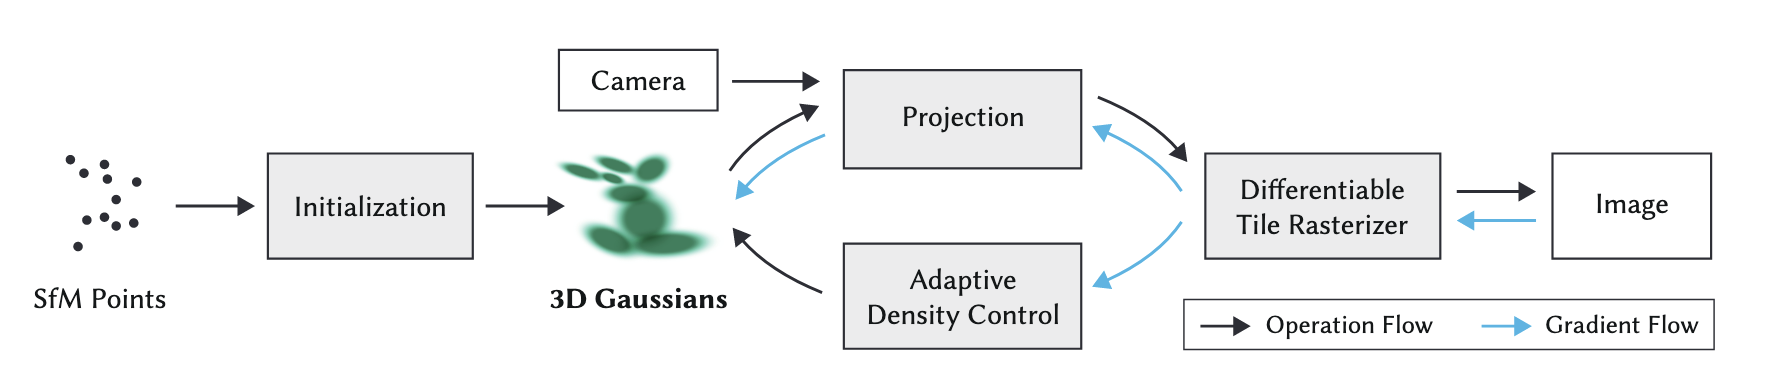
\includegraphics[width=\textwidth]{images/gs_process.png}
\caption{A diagram illustrating the Gaussian Splatting process from \cite{splat}}
\label{fig:gaussiansplatting}
\end{figure}

\section{Scaling NeRFs: Related work}

\subsection{Splitting NeRFs}

Neural radiance fields (\cite{nerf}) have been the state-of-the-art in view synthesis prior to gaussian splatting, and numerous works exist that try to scale the technique for larger scenes.

To address the same issue we are encountering regarding the memory limit, multiple smaller spatially segmented models have been used to represent scenes. In Block-NeRF (\cite{blocknerf}), which specifically aims to solve the issue of applying the NeRF technique in city scenes, the reconstruction space heuristically using city block boundaries. However its application is domain specific to the reconstruction of multiple city blocks. \cite{meganerf} later proposed using a geometric clustering algorithm to dynamically partition a scene into multiple smaller NeRF models by analyzing visibility statistics.

Inspired by the above techniques, we see that gaussian splatting could similarly benefit in being segmented into smaller models to make the reconstruction of larger scenes feasible. Furthermore, model segmentation in gaussian splatting should be even more straightforward because the parameters responsible of modeling the appearance of scenes can be spatially interpreted, and thus allows for directly segmenting gaussian splatting models after training.

\subsection{NeRFs for multi-scale reconstruction}

Other than just the practicality of scaling NeRFs to accommodate for computational power and memory limits, large scale scene reconstruction in learned representations also needs to consider the varying appearance of objects from different distances. Images of an object taken at a short distance may exhibit a high amount of detail, whereas images taken from further distances may have the object appear blurry, due to the finite amount of pixels in images. In the realm of NeRF training, \cite{bungeenerf} has proposed a coarse-to-fine training schedule, as well as a dynamically growing NeRF model in the form of residual blocks to allow for the progressive learning of higher detail at closer distances.

While gaussian splatting utilizes a different architecture to represent the scene, optimizing one model over images of the same object at drastically different scales may see similar issues, and thus this problem will also be something we put into consideration in the design of our technique.

\section{Scaling Structure from Motion: Related work}

Another similar problem would be the scaling of Structure from Motion (SfM) to larger datasets, which similarly may run into computational limits when scaled naively.

As a more mature field of research, numerous techniques have been explored in this space. \cite{spectral} proposed a novel technique that utilizes the Hessian of reprojection error and its eigenvectors to effectively factor the optimization into smaller problems, showing a theoretical interpretation on camera group clustering for the problem of SfM, and a technique that offers low residuals and can be efficiently computed. This clustering technique could potentially be applied in our optimization pipeline to quickly and effectively segment out camera camera groups.

Another paper, \cite{block}, explored dividing the problem into multiple groups based on the image adjacency matrix, demonstrating that the problem could be divided into smaller parallelizable problems.

Other works (\cite{hiercluster}, \cite{radcluster}, \cite{divideandconquer}) have hierachically splitting nested groups and then merging them back up in a bottom-up fashion, which have a provably lower computational complexity (\cite{hiercluster}).

\chapter{Proposed methods}

Given the variety of approaches to scaling NeRFs and SfM, in the exploratory stage, we should explore multiple approaches to scaling gaussian splatting training. The overarching theme is to divide the problem into smaller, more manageable problems, and then merging them back up to form a complete reconstruction.

However, it remains to be explored:
\begin{itemize}
\item How do we partition the problem into smaller problems?
\item How do we merge the smaller problems back up?
\item Should we partition recursively, or in a single pass?
\item How do we ensure the boundaries of the smaller problems are consistent?
\end{itemize}

Preliminarily, I am interested in recursive partitioning, because it may allow for the simultaneous generation of LOD models, which will be useful for subsequent LOD rendering. Moreover, we may dynamically change the depth of the recursive partitioning depending the computer's memory limit, such that even arbritarily large scenes could eventually be split into smaller problems that could fit into memory.

Drawing inspiration from \cite{bungeenerf}, we would also like to incorporate distance awareness in the process to model the varying appearance of objects at different distances more effectively, which will be useful for reconstructing multi-scale scenes. This requirement also fits well with the recursive partitioning approach, since we may utilize the distance of the camera to the object as part of the partitioning criteria to weigh coarser views more heavily for top level partitions, and closer views more heavily for lower level partitions. We are also drawing inspiration from \cite{spectral} to segment scenes with scene geometry in mind, which will reduce the amount of overlap between partitions and reduce artifacts.

Factoring in these considerations, here is a preliminary outline of building a pipeline we will explore. An overview is shown in Figure \ref{fig:gaussiansplattinglod}, but below is a more detailed description of certain steps of the pipeline.

\begin{figure}[h!]
    \centering
    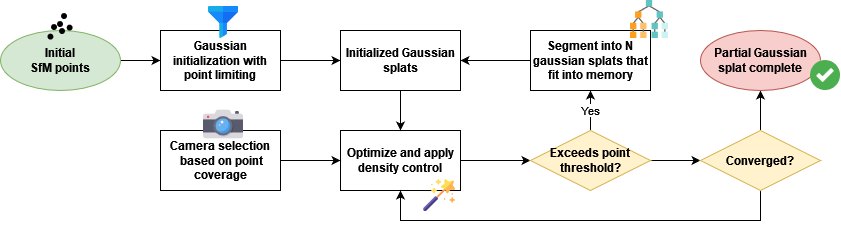
\includegraphics[width=\textwidth]{images/gslod_process.png}
    \caption{A flow diagram illustrating the proposed Gaussian Splatting LOD training process}
    \label{fig:gaussiansplattinglod}
\end{figure}

\subsection{SfM, Gaussian Splatting Initialization, and Camera Selection}
We assume SfM for the scene has already been performed, and thus we have a sparse point cloud of the scene, the camera parameters, and correspondances between the cameras and the points. We then initialize the gaussian splatting model using the sparse point cloud. However, unlike the original initialization process, we need to downsample the points to a size that would fit into memory. Moreover, we need to reduce the number of cameras to an amount that may still fit into memory, yet maximize the overall coverage of the downsampled points. As a side-effect, this reduces the amount of overlap and likely select cameras of the same scale.
\subsection{Gaussian Splatting Optimization and Paritioning}
Once we have the initial gaussian splatting model, we may then optimize the model using the same optimization process as the original gaussian splatting paper. However, since the optimization algorithm automatically grows the number of gaussians (and is likely to grow given we just downsampled the points), we will need to set a threshold for the maximum number of gaussians allowed in the model. Once the number of gaussians exceeds the threshold, we will need to partition the model into smaller models.
\subsection{Recursive Partitioning}
In partitioning the model into smaller models, we would desire the following properties:
\begin{itemize}
    \item The smaller models are of similar size, and thus can more effectively fit into memory
    \item The smaller models' camera coverage of points should be orthogonal to each other, such that the smaller models can be merged back up without artifacts
\end{itemize}
We suggest representing cameras as a graph, where each camera is a node, and the edges between the nodes represent the amount of overlap between the cameras. We may then use the spectral graph partitioning algorithm with balanced partitioning constraints to partition the cameras into smaller groups (see \cite{bgraph}). 

\section{Efficient algorithms for dealing with large spatial datasets}

Implementationally, using such techniques for gaussian splatting reconstructions pose unique challenges, because in order to train gaussian splatting models, it needs to fit on the GPU; on the other hand, the process of splitting gaussian splats may be more suitable for the CPU due to the complexities of running data structures required to effectively filter and segment large gaussian splats.

Moreover, the merged results of multiple gaussian splatting reconstruction may not fit in GPU memory, and will need to be stored either on the CPU or on disk. Fortunately, gaussian splats could be easily represented as a regular point cloud with extra attributes, and for the task of manipulating and storing massive gaussian splats that could not fit on memory, we can simply leverage the mature field of point cloud research for existing tools (\cite{pcl}, \cite{cilantro}). However we do need to write an efficient enough interchange that readily moves gaussian splats between these data structures and the GPU, when switching between splat optimization, and manipulating and storing splats.

\chapter{Research Roadmap}

The following roadmap outlines the systematic approach that will be undertaken to carry out research for the dissertation:

\begin{itemize}
\item Comprehensive Evaluation: Begin by assessing Gaussian splatting's performance on large multi-scale scenes. Through this evaluation, we aim to identify and document instances where Gaussian splatting falls short or exhibits failure cases.

\item Optimization Analysis: Undertake a rigorous investigation to determine the bottlenecks in the current optimization process. This will guide subsequent modifications and enhancements.

\item Out-of-Core Database Development: Construct an out-of-core database infrastructure to facilitate seamless transformation between differentiable and non-differentiable formats. Our preliminary focus is on the interoperability between PCL and PyTorch.

\item Recursive Partitioning: Implement a method for recursively splitting the scene during the reconstruction process. This is pivotal to managing and optimizing larger scenes more efficiently.

\item Merging Technique Development: Post recursive splitting, devise a mechanism to merge the partitioned segments, ensuring consistency and accuracy in the final reconstructed scene.

\item Visualization Creation: Generate rudimentary visualizations of the reconstructions. These visualizations will be instrumental in visually assessing the quality, accuracy, and efficiency of the proposed methods.
\end{itemize}

\section{Evaluation Metrics for Dissertation Success}

The dissertation's accomplishments will be measured through a combination of quantitative and qualitative assessments. These metrics will ensure a holistic evaluation of the innovations and optimizations proposed in the context of Gaussian splatting for large-scale view synthesis.

\subsection{Quantitative Metrics}

\begin{enumerate}
    \item \textbf{Memory Usage Reduction}:
    \begin{itemize}
        \item \textit{Method}: Quantitatively compare the memory utilization of the standard Gaussian splatting methodology with the proposed optimized technique using the same input dataset.
        \item \textit{Success Criteria}: A noticeable diminution in memory footprint while retaining the synthesized view's fidelity.
    \end{itemize}

    \item \textbf{Processing Speed}:
    \begin{itemize}
        \item \textit{Method}: Quantify the time consumption for view synthesis between conventional and optimized techniques.
        \item \textit{Success Criteria}: Either a speed enhancement or a time performance parity, ensuring no compromise due to memory optimizations.
    \end{itemize}

    \item \textbf{Quality of Synthesized Views}:
    \begin{itemize}
        \item \textit{Method}: Implement renowned image quality metrics such as PSNR, SSIM, and MSE to benchmark the quality of generated views.
        \item \textit{Success Criteria}: Scores reflecting that the proposed technique's output either matches or surpasses the traditional method.
    \end{itemize}
\end{enumerate}

\subsection{Qualitative Metrics}

\begin{enumerate}
    \item \textbf{Expert Reviews}:
    \begin{itemize}
        \item \textit{Method}: Solicit feedback on synthesized views from computer graphics connoisseurs.
        \item \textit{Success Criteria}: Affirmative responses emphasizing the visual quality and appeal of the optimized technique.
    \end{itemize}

   %  \item \textbf{Usability of Web-based Viewer (if developed)}:
   %  \begin{itemize}
   %      \item \textit{Method}: Execute usability assessments with users to gauge their experience with the proposed viewer.
   %      \item \textit{Success Criteria}: Positive user experiences and testimonials regarding the viewer's functionality.
   %  \end{itemize}
\end{enumerate}

\subsection{Practicality and Applicability}

\begin{enumerate}
    \item \textbf{Integration with Existing Libraries}:
    \begin{itemize}
        \item \textit{Method}: Document assimilating the optimized technique into prevailing libraries.
        \item \textit{Success Criteria}: An uncomplicated integration procedure, underscoring the proposed method's adaptability.
    \end{itemize}

    \item \textbf{Scalability Test}:
    \begin{itemize}
        \item \textit{Method}: Evaluate the technique's robustness and performance across diverse dataset magnitudes.
        \item \textit{Success Criteria}: Consistent augmentation in performance and memory conservation as data complexity escalates.
    \end{itemize}
\end{enumerate}

\chapter{Additional Research Directions}

Beyond our primary research objectives, should our timeline permit, we are eager to explore several supplementary avenues that could significantly enhance the depth and breadth of our investigation.

\section{Integration with NeRF Techniques}

One area of promise lies in the potential to combine NeRF-related techniques with Gaussian splatting, especially when modeling distant objects. Gaussian models have frequently shown shortcomings when tasked with reconstructing expansive terrains such as the sky. This is primarily because the inherent featurelessness of such areas offers scant Structure from Motion (SfM) points to fit Gaussians accurately.

This challenge is further compounded by the fact that Gaussians struggle with representing objects positioned at infinite distances or those lacking a well-defined structure. Against this backdrop, we hypothesize that a dual-model approach might be beneficial. Here, Gaussian splatting could focus on proximate objects, while another distinct representation hones in on more distant subjects. This hybrid approach could potentially refine the function of traditional graphics skyboxes by endowing them with enhanced view-dependent properties.

\section{Web-Based Gaussian Splat Visualization}

Another intriguing proposition is the development of a web-based viewer for visualizing Gaussian splats with Levels of Detail (LODs). While this might seem straightforward on the surface, the process is replete with challenges.

For instance, we would require a data storage format that enables pinpointed retrieval of specific levels or segments. An octree format, potentially building upon the pioneering work of Potree (\cite{potree}), emerges as a likely candidate.

Then there is the matter of crafting an order-independent transparency that remains consistent across web platforms (\cite{webglsplat}).

Finally, the viewer has to intelligently selecting the right LOD, as well as ensuring seamless transitions between different LODs, and it’s evident that the task at hand is far from simple.

\chapter{Conclusion}

In closing, while Gaussian splatting enables unparalleled quality in view synthesis, scaling it to large scenes poses severe memory challenges. Our solution entails an out-of-core optimization pipeline, leveraging techniques like recursive partitioning and merging. This will push reconstructions to unprecedented scales.

We will comprehensively evaluate current limitations, analyze optimization bottlenecks, develop out-of-core infrastructure, implement recursive splitting and merging algorithms, and generate visualizations. Beyond our core objectives, integrating Gaussian splatting with NeRF and building an interactive LOD viewer are exciting avenues for exploration.

In summary, this undertaking promises to unlock Gaussian splatting's true potential for expansive scene reconstruction via pioneering out-of-core innovations. We look forward to systematically overcoming existing barriers to facilitate reconstructions previously impossible. The project will be both academically impactful and graphically groundbreaking as we drive Gaussian splatting to new frontiers.


% \bibliographystyle{plain}
\bibliographystyle{plainnat}
\bibliography{mybibfile}


% % You may delete everything from \appendix up to \end{document} if you don't need it.
% \appendix

% \chapter{First appendix}

% \section{First section}

% Any appendices, including any required ethics information, should be included
% after the references.

% Markers do not have to consider appendices. Make sure that your contributions
% are made clear in the main body of the dissertation (within the page limit).

% \chapter{Participants' information sheet}

% If you had human participants, include key information that they were given in
% an appendix, and point to it from the ethics declaration.

% \chapter{Participants' consent form}

% If you had human participants, include information about how consent was
% gathered in an appendix, and point to it from the ethics declaration.
% This information is often a copy of a consent form.


\end{document}
